\documentclass[11pt]{article}
\usepackage[margin=1in]{geometry}
\usepackage{graphicx}
\begin{document}
\section*{R93 principal-open overlap: rejected attempt}
The frozen \texttt{overlap93-01} attempt was rejected by the strict
driver. Seven of seven named functions reached polynomial rank-32
membership lines, but the coefficient inversion step called
\texttt{lift} on the base-field coefficient \texttt{u}. Singular
reported native errors while still exiting zero and printing a pass
marker. The acceptance rule correctly rejected the result.

\begin{center}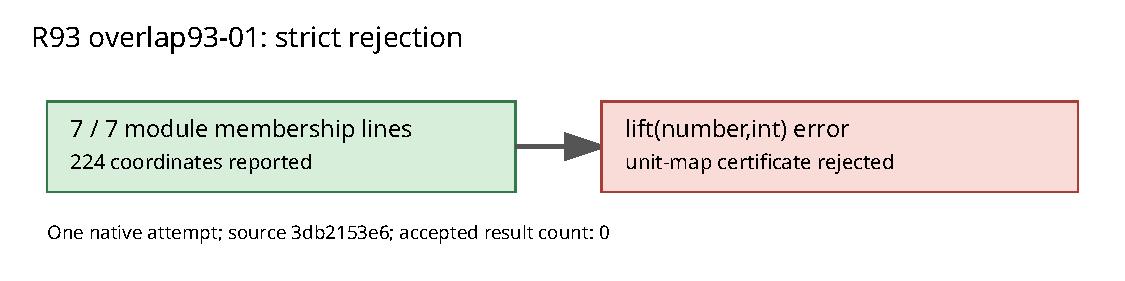
\includegraphics[width=.9\textwidth]{diagram.pdf}\end{center}

The next attempt will use direct \texttt{1/u} coefficient inversion
in a newly frozen source. No chart-gluing claim is taken from R93.
See \texttt{CM.md}, the raw native log, and the preserved source hashes.
\end{document}
